\chapter{Cache Mechanisms}

Caching faces complex concerns:  delay, synonym detection, the precise manner
of tagging, security issues such as seen in recent speculative execution
vulnerabilities, and more.

\section{NCOR}

In 2012, Aasaraai and Moshovos published "NCOR:  An FPGA-Friendly Nonblocking
Data Cache for Soft Processors with Runahead Execution."  Nonblocking cache
allows instruction-level parallelism and specifically allows runahead
execution, wherein a CPU waiting for a cache miss—possibly long enough to
execute several tens or hundreds of instructions—can run instructions with
incorrect data and discard the results just to figure out what data will be
fetched.  A load-store architecture like RISC-V accesses memory infrequently
while executing, so long as the instruction cache can provide the next several
instructions.  Runahead discards the results of instructions, but queues data
cache loads as best it can predict so they occur while the CPU executes
preceding instructions.  Runahead can often generate confirmed correct
computations, notably for branches, providing a high-accuracy branch predictor.

Runahead does particularly interesting things when encountering loops:  if it
can properly predict valid load addresses within the loop—such as by tracking
an increment—it can rapidly identify further data with high accuracy.  If
runahead produces erroneous results, a cache miss will occur when entering the
loop; once inside the loop, this information is definitely correct, and
runahead generally predicts the correct results.

NCOR provides a non-blocking cache which avoids content-addressable memory and
leverages FPGA resources such as BRAM.  It reaches fMax of over 325MHz on a
Spartan III with a 4KiB cache, versus 200MHz for a stripped-down MSHR-based
cache.  Both architectures spend more time slogging through larger caches, with
NCOR running at 300MHz on both 8KiB and 16KiB cache sizes, and near 275MHz on
32KiB.  Separate instruction and data caches with slower (multi-cycle, low
delay but longer latency) L2 cache allow higher fMax when the cache
infrastructure is in the critical path, which means more runahead distance and
fewer cache misses.

\section{VC-DSR}

Most L1 caches are virtually-indexed, physically-tagged (VIPT).  This requires
a TLB lookup on each cache access, possible page table walking, and other slow
behavior.  The TLB lookup itself induces longer delays.  Virtually-indexed,
virtually-tagged (VIVT) caches can encounter multiple virtual addresses (VAs)
with the same physical address, called synonyms.

Yoon and Sohi proposed\footcite{Yoon2016} a Virtual Cache with Dynamic Synonym
Remapping (VC-DSR), as shown in \prettyref{fig:VC-DSR}.  This solves the
synonym probleh in VIVT by looking up synonyms in an Active Synonym Table (AST)
if a virtual address matches a Synonym Signature (SS), implemented as a bloom
filter.  If no SS or AST hit, it checks the VC as normal.  When multiple cached
virtual pages map to the same physical page, the AST provides the Leading
Virtual Page (LVP) used to look up the address in the VC, as well as the
permissions and other metadata for that particular virtual page.  The cache
then looks up the tag for the leading virtual page—logically, it replaces the
bits in the virtual address with the bits of the leading virtual page,
producing the Leading Virtual Address (LVA), and uses that to find the cache
line; the L1 arbiter ignores the metadata in this cache entry, using the data
from the AST instead.

\begin{figure}[hbpt]
    \centering
    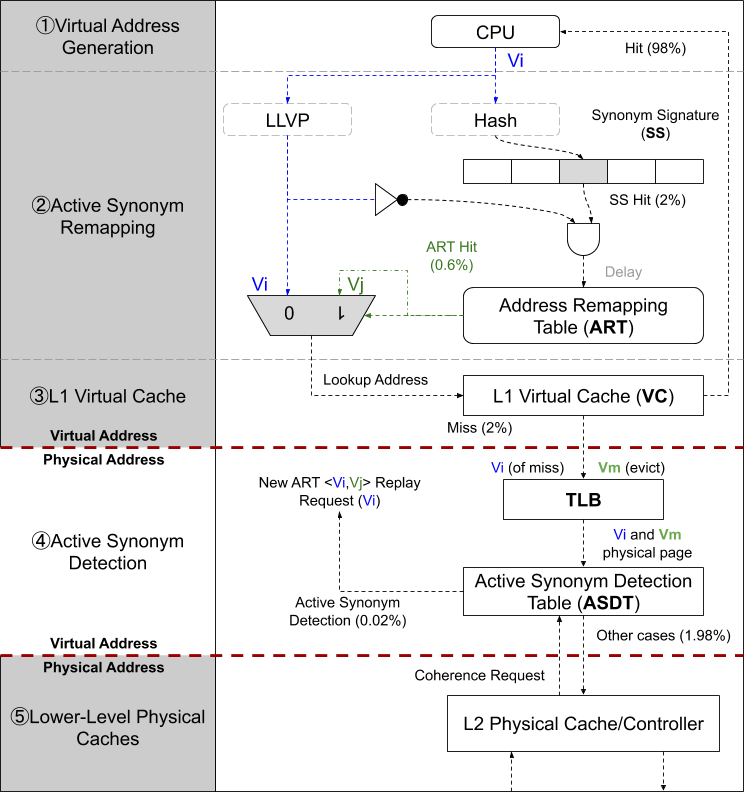
\includegraphics[width=\textwidth]{images/VC-DSR_Cache}
    \caption{\label{fig:VC-DSR}VC-DSR as diagramed by Yoon and Sohi, with LLVP added.}
\end{figure}

On VC miss, the TLB checks the Active Synonym Detection Table (ASDT) to
determine if the virtual page is known to correspond to a physical page in
cache.  If not, the caching system makes further requests to L2 cache or
performs a page table walk.  If the virtual page ultimately does reference a
physical page already in cache, the cache arbiter hashes the page, sets the
corresponding bit in SS, increments a counter for this bit, and inserts the
virtual page into the AST as a synonym to the LVP.

The Last LVP (LLVP) optimization, shown in \prettyref{fig:VC-DSR}, stores the
last leading virtual page and requested page in a register, along with
metadata.  If the requested address matches the last requested address, the
cache arbiter can immediately check metadata (read or write permission) and mux
the LVP from this register.  Consecutive memory accesses to the same synonym
page skip the AST check; the SS check occurs in parallel, but adds no delay and
has no effect.

RISC-V provides a Global bit in the PTE.  The cache arbiter ignores the ASID
for Global pages, placing no entry in the SS or AST for the same virtual page
in different ASIDs.  Synonyms mapped at alternate virtual addresses are treated
as normal.  On IA-32 and AMD64, Yoon and Sohi assume the top half of virtual
address space is global.
